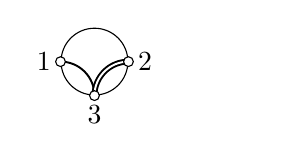
\begin{tikzpicture}
  [ scale = 0.6,
    thin,
    inner/.style={circle,draw=black!100,fill=black!100,inner sep=1.25pt},
    attach/.style={circle,draw=black!100,fill=black!0,thin,inner sep=1.25pt},
    sin/.style={line width=.7pt},
    doub/.style={line width=2.1pt},
    trip/.style={draw=white,line width=.7pt}]
    \node at (0,0){};
%\begin{scope}[yshift=1.8cm]
%  \node (2)  at (0,0) [attach,label=left:3] {};
%  \node (1)  at (0,1) [attach,label=left:1] {};
%  \node (3)  at (3,1) [attach,label=right:2] {};
%  \node (4)  at (1,0) [inner]  {};
%  \node (5)  at (2,0) [inner]  {};
%  \node (6)  at (1,1) [inner]  {};
%  \node (7)  at (2,1) [inner]  {};
%  \node (8)  at (2,2) [inner]  {};
%  \node (9)  at (2.866,2.5)  [inner] {};
%  \node (10) at (1.134,2.5)  [inner] {};
%  \node (11) at (2,-1)       [inner] {};
%  \node (12) at (2.866,-1.5) [inner] {};
%  \node (13) at (1.134,-1.5) [inner] {};
%
%  \draw (2) to (4);
%  \draw (4) to (5);
%  \draw (3) to (7);
%  \draw (1) to (6);
%  \draw (6) to (4);
%  \draw (6) to (7);
%  \draw (7) to (5);
%  \draw (7) to (8);
%  \draw (8) to (9);
%  \draw (8) to (10);
%  \draw (11) to (5);
%  \draw (11) to (12);
%  \draw (11) to (13);
%
  \node (split) at (-3.6,.8) [draw=black,circle,inner sep=3mm,
         label=left:1,label=right:2,label=below:3] {};
% 
%  \node at (-1.6,.5) {=};

  \draw[sin]  (split.west) to[out=0,in=90]   (split.south);
  \draw[doub] (split.east) to[out=180,in=90] (split.south);
  \draw[trip] (split.east) to[out=180,in=90] (split.south);
  
  \node at (split.east) [attach] {};
  \node at (split.west) [attach] {};
  \node at (split.south) [attach]{};
%\end{scope}
\end{tikzpicture}